\begin{frame}
    \frametitle{Frequency response}
    \begin{itemize}
        \item Input frequency from \SIrange{1}{900}{Hz}
        \item Compare using maximum displacement
    \end{itemize}
    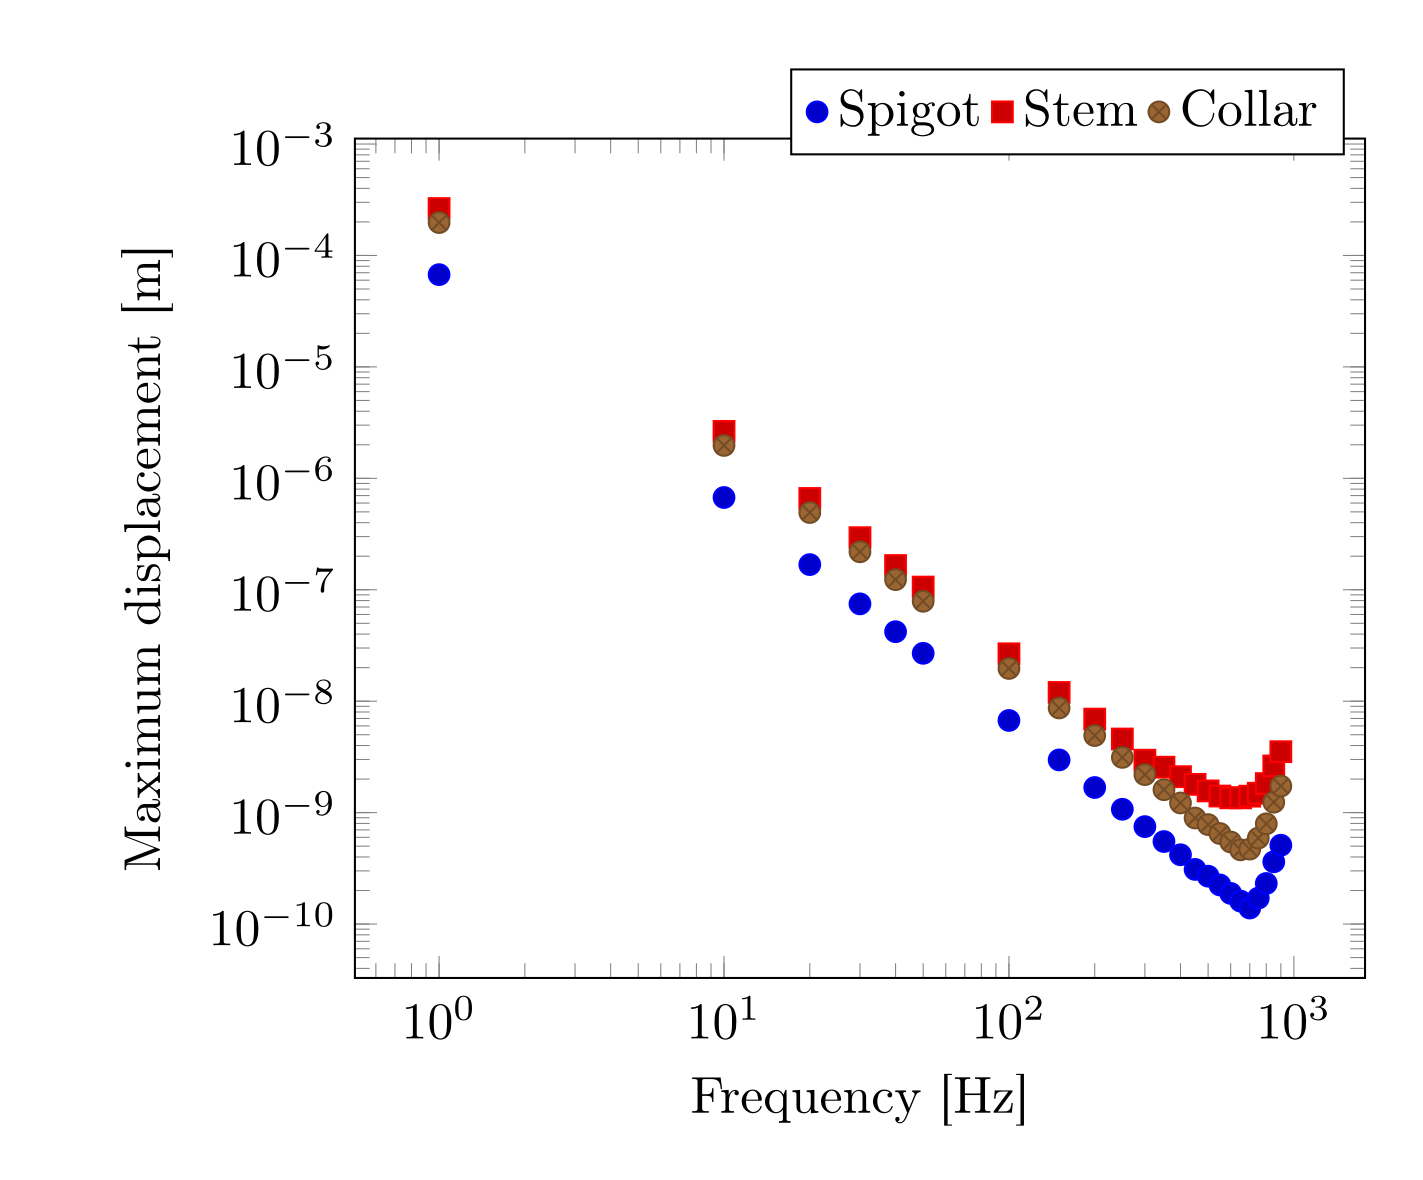
\includegraphics[width=0.45\textwidth]{figures/frequency-response.png}
    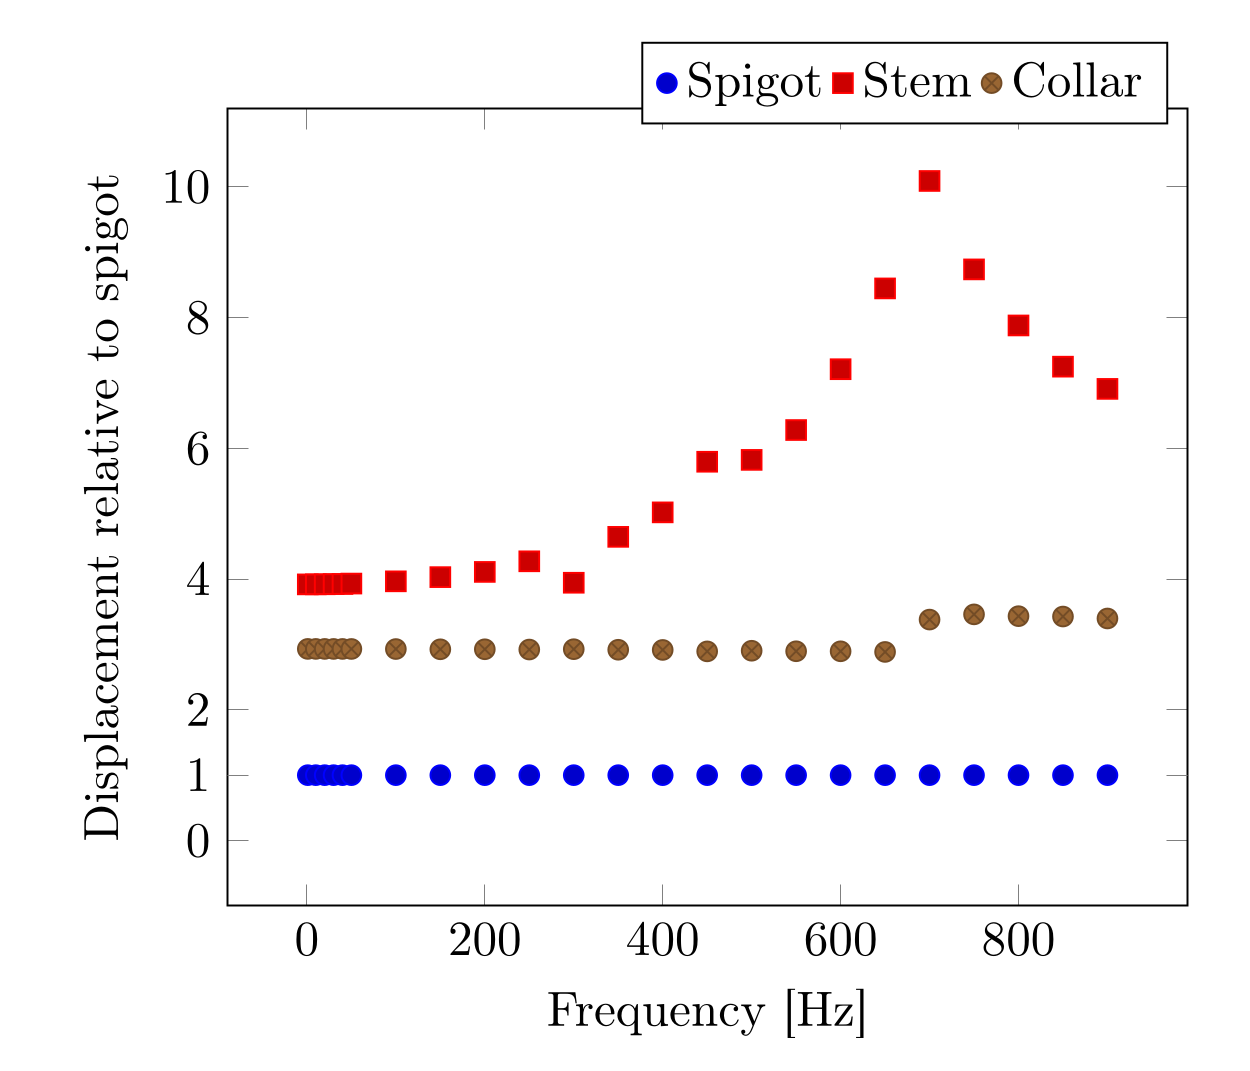
\includegraphics[width=0.45\textwidth]{figures/frequency-response-relative.png}
    

\end{frame}

\begin{frame}
    \frametitle{Time-variance}

    \begin{itemize}
        \item Displacement in the direction of the load:
    \end{itemize}
    \begin{center}
        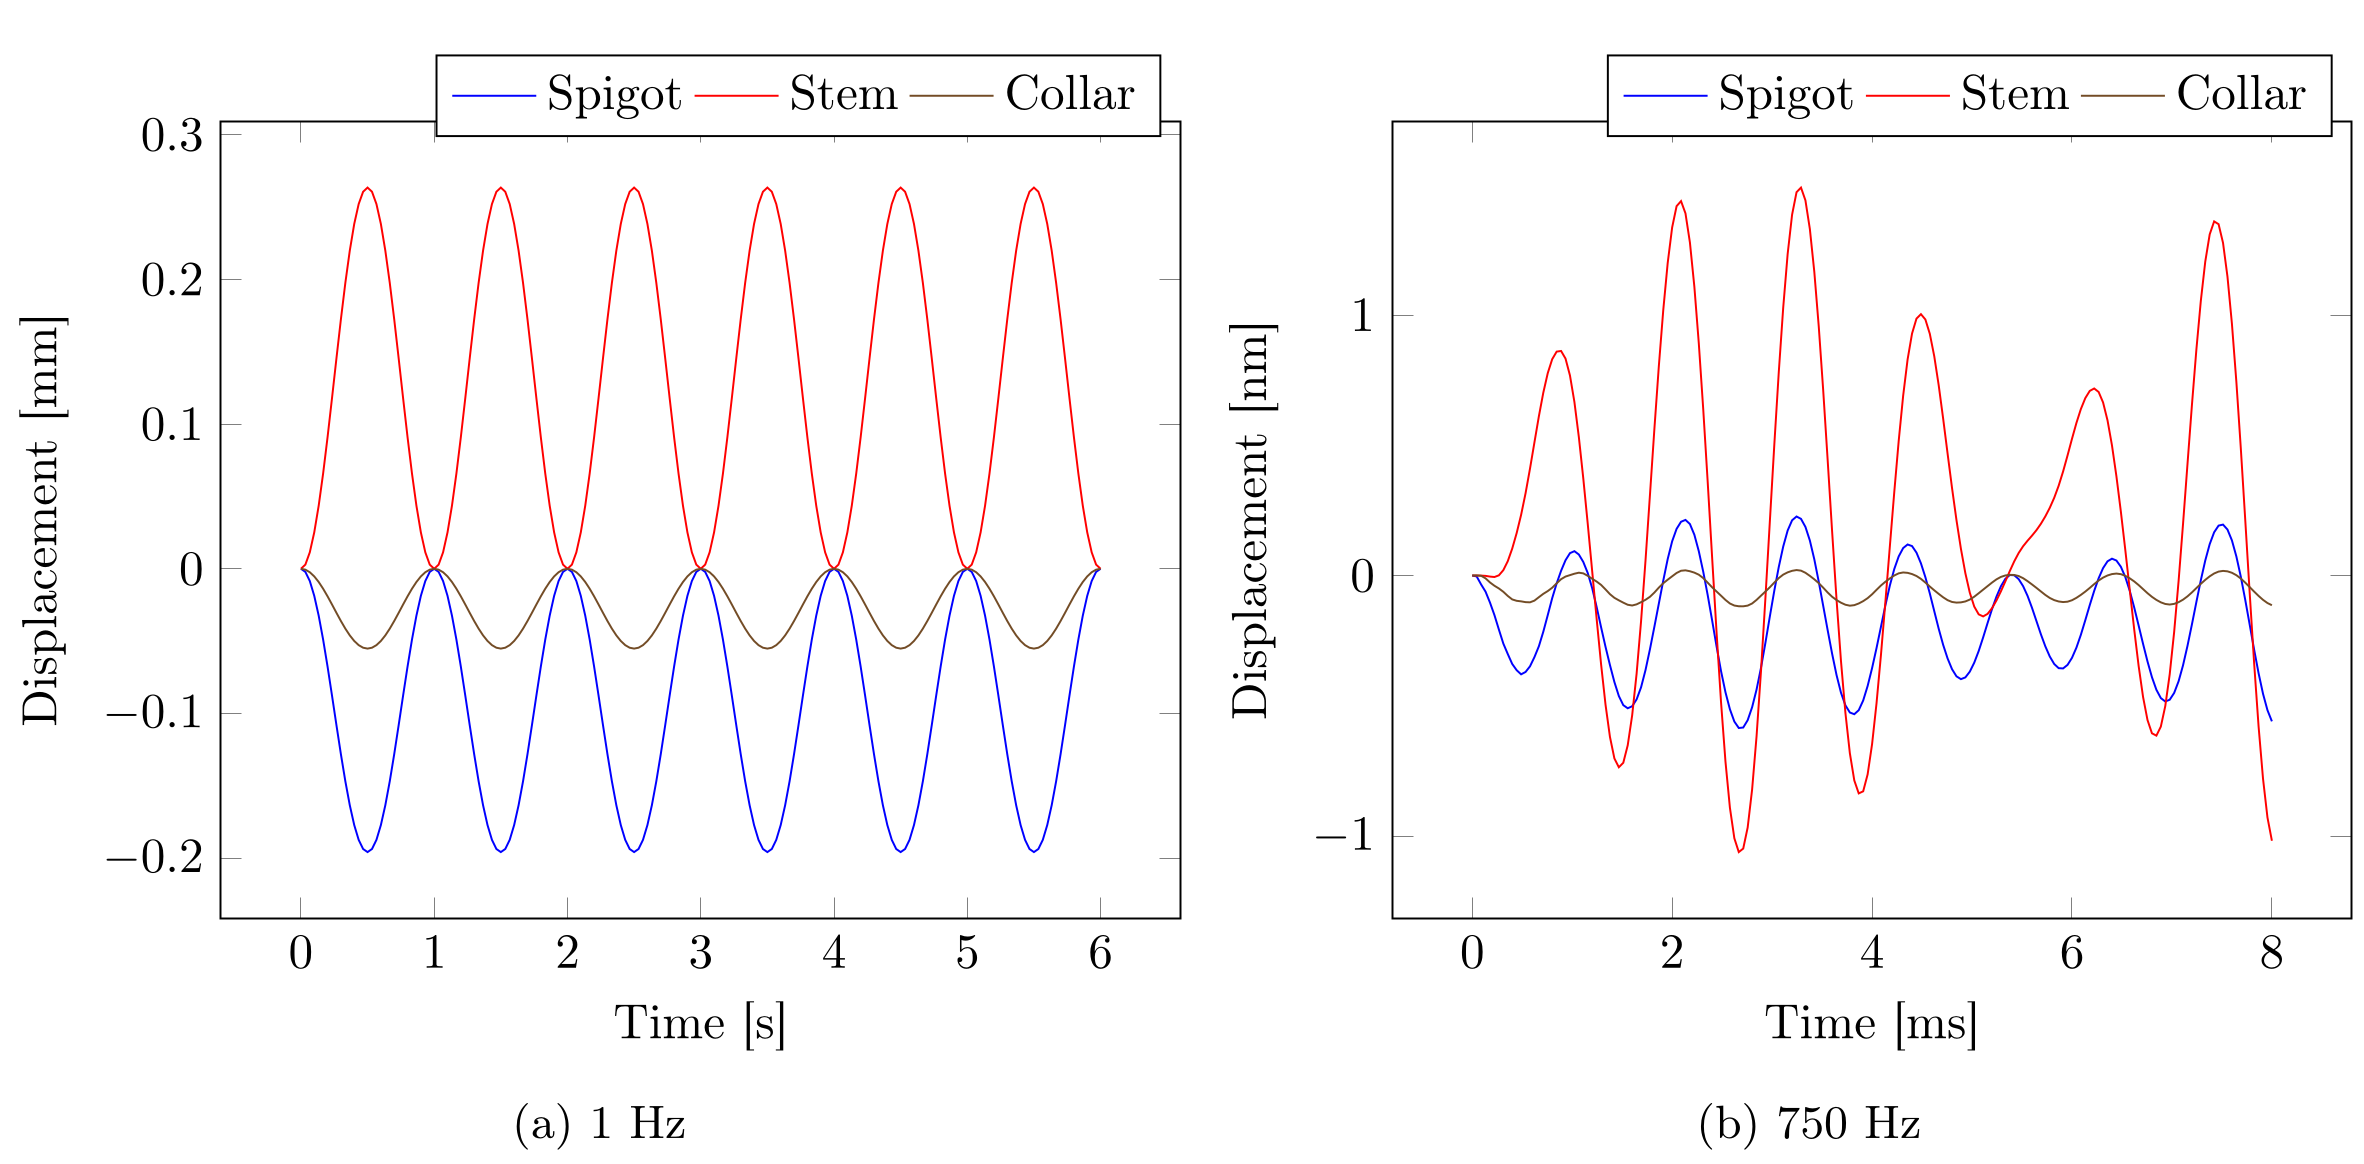
\includegraphics[width=0.8\textwidth]{figures/displacement-over-time.png}
    \end{center}
    \begin{itemize}
        \item At low frequencies: Time-invariant
        \item At high frequencies: Time-variant
    \end{itemize}
\end{frame}

\begin{frame}
    \frametitle{Quantifying change over time}
    \begin{itemize}
        \item Run simulations for 500 periods
        \item First 100 periods for \SI{750}{Hz}:
    \end{itemize}
    \begin{center}
        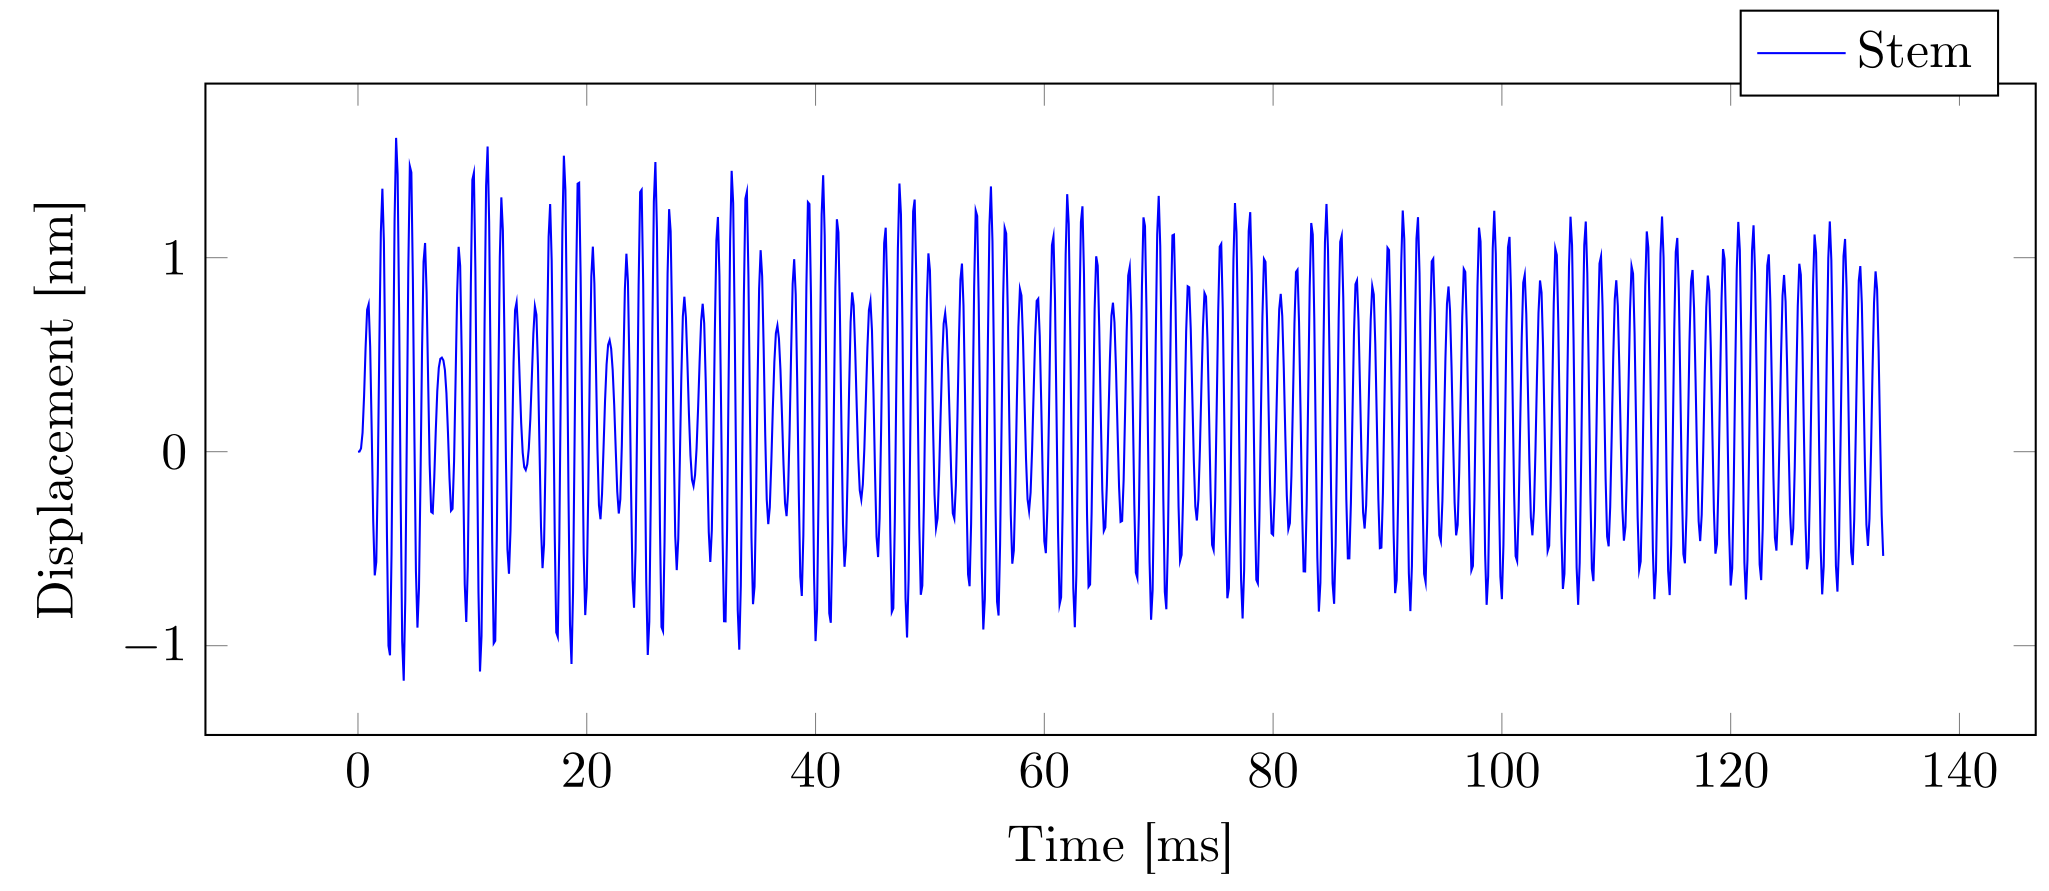
\includegraphics[width=0.9\textwidth]{figures/750hz-100-periods-time.png}
    \end{center}
    \begin{itemize}
        \item Hard to quantify when it stops changing with time
    \end{itemize}
\end{frame}

\begin{frame}
    \frametitle{Quantifying change over time}
    \begin{itemize}
        \item Compare local maxima with global maximum
        \item Spigot and collar have amplitude loss:
    \end{itemize}
    \begin{center}
        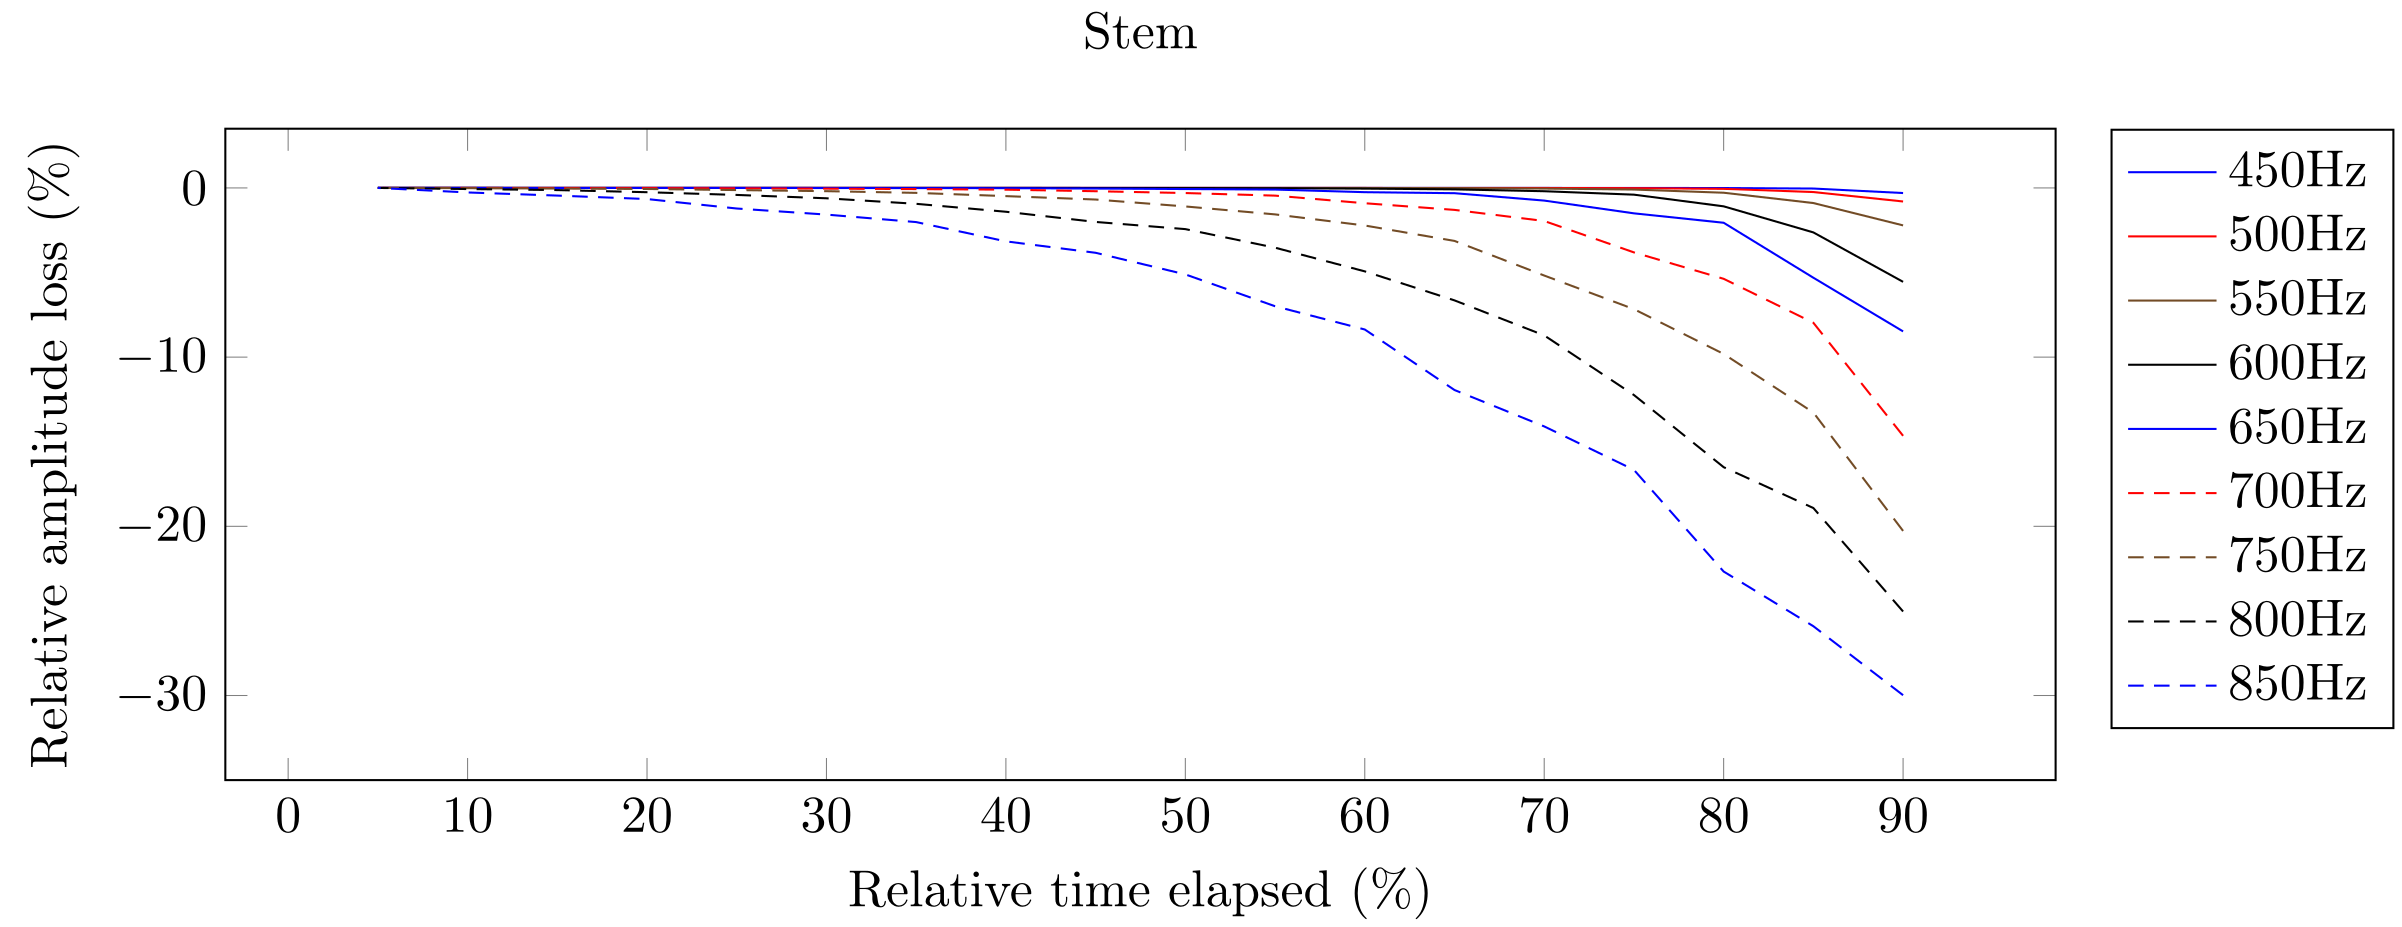
\includegraphics[width=0.9\textwidth]{figures/relative-amplitude-decrease.png}
    \end{center}

\end{frame}

\begin{frame}
    \frametitle{What does this information tell us?}
    \begin{itemize}
        \item Control amplitude of vibrations using combination of: \begin{itemize}
            \item Frequency
            \item Position of actuator
            \item Amplitude of impulse
        \end{itemize}
        \item Quantified how vibrations propagate through ITAP
    \end{itemize}
\end{frame}

\begin{frame}
    \frametitle{How good is our model?}

    \begin{center}
        \alt<1>{
            \begin{columns}
                \begin{column}{0.5\textwidth}
                    \begin{itemize}
                        \item F: ``Flanged'', more complete model
                    \end{itemize}
                    \begin{center}
                        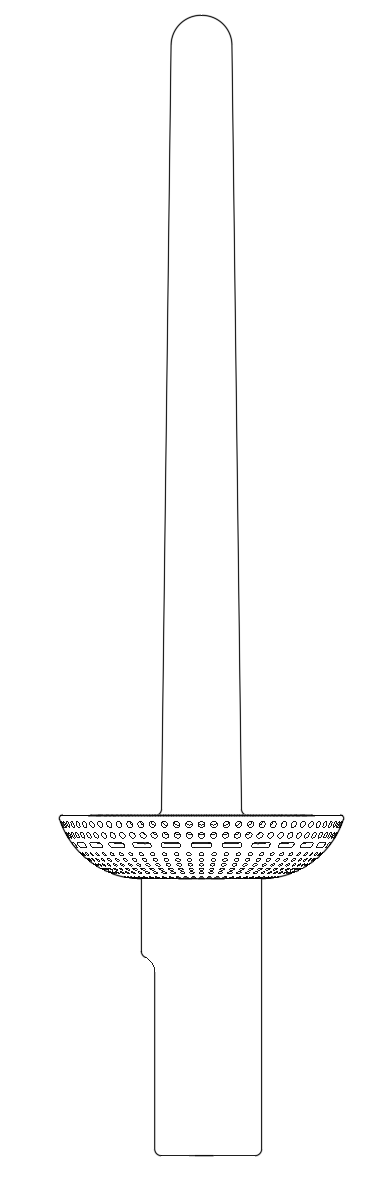
\includegraphics[height = 5cm]{figures/itap-complex.png}
                    \end{center}
                \end{column}
                \begin{column}{0.5\textwidth}
                    \begin{itemize}
                        \item S: Simplified model used in these simulations
                    \end{itemize}
                    \begin{center}
                        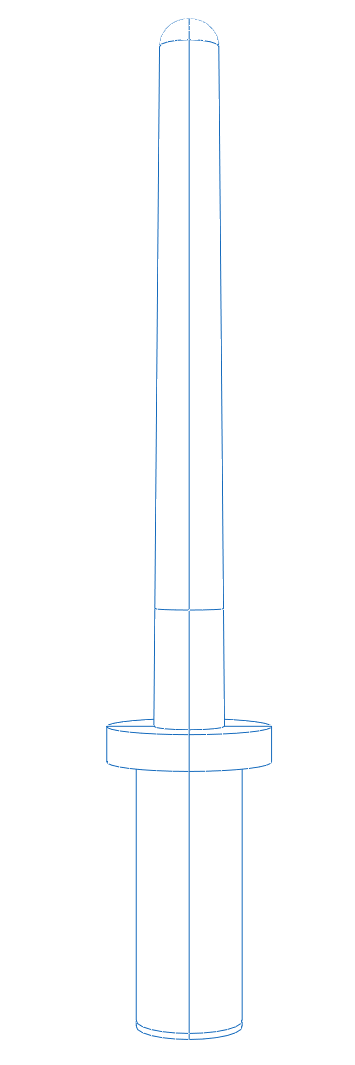
\includegraphics[height = 5cm]{figures/itap-simplified.png}
                    \end{center}
                \end{column}
            \end{columns}
        }{}
        \alt<2>{
            \begin{itemize}
                \item F: ``Flanged'', more complete model
                \item S: Simplified model used in these simulations
                \item Error of 0 is ideal.
            \end{itemize}
            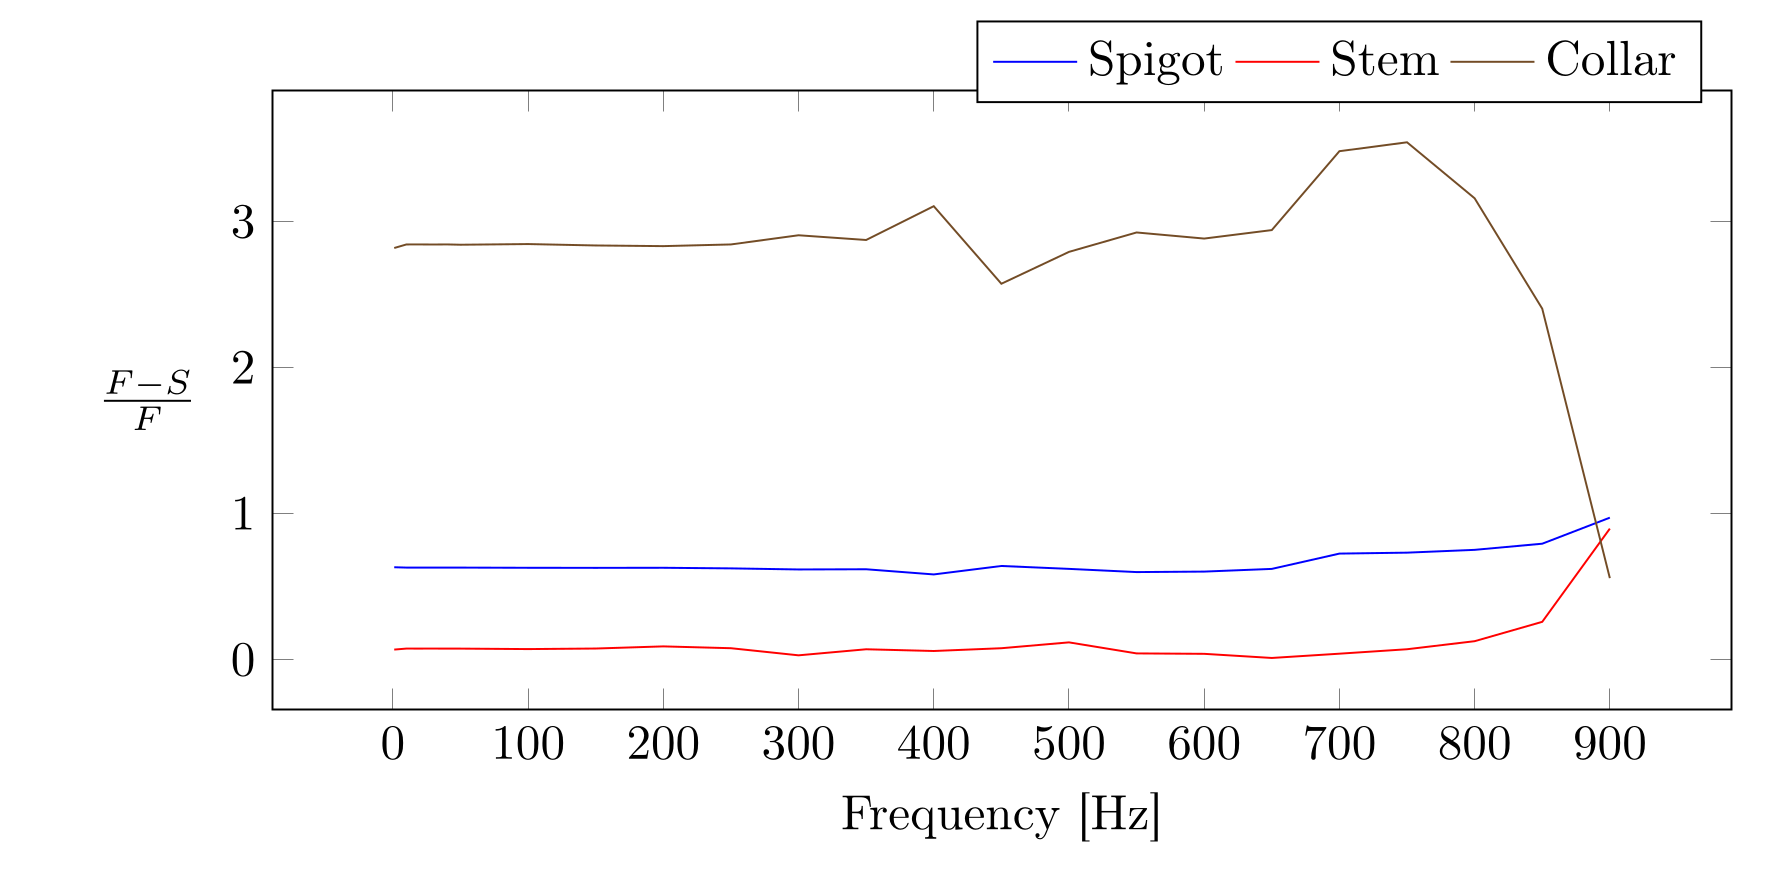
\includegraphics[width=0.9\textwidth]{figures/error.png}
        }{}
    \end{center}
\end{frame}